\documentclass[11pt]{article}

\usepackage[margin=0.85in]{geometry}
\usepackage{amsmath}
\usepackage{amssymb}
\usepackage{booktabs}
\usepackage{xcolor}
\usepackage{microtype}
\usepackage{graphicx}
\usepackage{tikz}
\usepackage{float}
\usepackage{array}
\usepackage{url}
\usetikzlibrary{arrows.meta,calc,fit,positioning,shapes.geometric}

\definecolor{forwardblue}{RGB}{37,99,235}
\definecolor{backred}{RGB}{190,18,60}
\definecolor{writeorange}{RGB}{217,119,6}
\definecolor{stategreen}{RGB}{22,101,52}
\definecolor{lightgray}{RGB}{246,247,249}

\newcommand{\code}[1]{\texttt{#1}}
\newcommand{\vstate}[1]{\ensuremath{V_{\mathrm{#1}}}}

\title{Toward Fully On-Device SPICE Training of a Local-Feature MNIST Network}
\author{SPICENN architecture note}
\date{\today}

\begin{document}
\maketitle

\begin{abstract}
This note documents the SPICENN circuit architecture that currently works and
the gap that remains.  The present deck is a phase-resolved local-feature
readout network trained in one uninterrupted SPICE transient: Python supplies
only external input rails, target rails, clock/control waveforms, and final
diagnostics.  It does not read hidden state, write weights, replay reference
updates, or checkpoint neural-network state between samples.  On MNIST, a
random-initialized \(10\times 10\), block-4, stride-2, 2-channel network trained
for 6000 online updates with \(\mathrm{batch\_size}=1\) reached \(90.15\%\)
accuracy on the full 10,000-image test set, improving from a \(10.89\%\)
random baseline.

That run is not the final goal.  It used behavioral SPICE current equations for
the neuron storage and writer cells, and it used a local-PCA sample ordering
chosen to reduce input waveform switching.  The result is therefore best read
as strong architectural evidence for capacitor-held state and phase-gated
local updates, not as a completed fully device-level training demonstration.
The remaining goal is a random-init, one-transient, \(\mathrm{batch\_size}=1\)
SPICE training run with realistic sample order, no Python neural-state
updates/checkpoints, device-level neuron/write circuits, and full 10,000-image
MNIST accuracy above \(90\%\).
\end{abstract}

\section{Contract}

The target contract is narrower and stronger than ``SPICE was used somewhere
in the loop.''  During a training run:
\begin{enumerate}
  \item Python chooses the sample sequence and drives input, label, clock, and
    scalar control waveforms.
  \item All trainable neural state remains inside one SPICE transient.
  \item Each sample is processed online with \(\mathrm{batch\_size}=1\).
  \item Python does not compute hidden activations, deltas, or weight updates.
  \item Python does not checkpoint or rewrite network state between samples.
  \item The only post-run readout is diagnostic: final capacitor voltages are
    measured and evaluated for accuracy.
\end{enumerate}

The 6000-update local-PCA run satisfies this execution contract: it uses one
Xyce transient, no reference replay, and no Python-side neural-state updates.
The final 10,000-image evaluation is a NumPy diagnostic of the SPICE-trained
final state.  The training trajectory itself is not computed by NumPy or by a
Python optimizer.

This execution contract is necessary but not sufficient for the full objective.
A final-goal result must also remove unrealistic training-order assumptions and
replace the behavioral neuron/write kernels with device-level circuits or
validated transistor subcircuits.

\section{Basic Building Blocks}

The working deck is still built from a small set of circuit-level ideas.  Some
are literal passive/state elements; others are behavioral current sources that
stand in for transistor subcircuits while the architecture is being validated.

\begin{center}
  \begin{tabular}{>{\raggedright\arraybackslash}p{0.27\linewidth}>{\raggedright\arraybackslash}p{0.62\linewidth}}
    \toprule
    Block & Role in the current deck \\
    \midrule
    Capacitor state &
    A voltage on a capacitor is the persistent neural state.  Local feature
    weights \(W_{bcp}\), local biases \(b_{bc}\), hidden activations \(h_{bc}\),
    hidden deltas \(\delta h_{bc}\), and readout weights \(V_{kbc}\) are all
    represented as node voltages. \\
    \addlinespace
    PWL input/target rails &
    Python drives external pixel and label waveforms.  These are inputs to the
    experiment, not computed neural state. \\
    \addlinespace
    Phase rails &
    Global rails such as activation-store, score-store, error/backward, and
    accumulation/write open local current paths at known times.  The
    high-accuracy behavioral run uses pulse-gated clocks to avoid long explicit
    PWL clock tables. \\
    \addlinespace
    Behavioral transconductor &
    A SPICE \(B\)-source current term relaxes a storage capacitor toward a
    local expression, e.g. \(h\leftarrow\tanh(z)\), only while the matching
    phase rail is high.  This is the validated architectural stand-in for the
    eventual transistor neuron/write cell. \\
    \addlinespace
    Signed rail pair &
    Signed quantities require differential or equivalent positive/negative
    storage.  Even if an activation is nonnegative, preactivations, synapse
    contributions, errors, hidden deltas, and writes are signed. \\
    \bottomrule
  \end{tabular}
\end{center}

The important distinction is that the current evidence is not a software
checkpoint loop.  The behavioral current sources are inside one SPICE transient
and act on capacitor voltages continuously over time.  Python only prepares the
external waveforms and reads the final state for diagnostics.

\section{Working Architecture}

The best explored network is a local-feature classifier rather than a dense CNN.
MNIST images are resized to \(10\times 10\) and quantized to 16 input levels.
The trainable hidden layer uses all \(4\times4\) spatial blocks at stride 2.
For a \(10\times10\) image this gives
\[
  \left(\frac{10-4}{2}+1\right)^2 = 16
\]
block positions.  Each block owns two independent local feature channels, so
the hidden representation has \(16\times2=32\) feature states.  A 10-class
readout maps those 32 feature activations to class scores.

The phrase \(\code{10x10 b4 stride2 c2}\) therefore means:
\begin{center}
  \begin{tabular}{ll}
    \toprule
    Token & Meaning \\
    \midrule
    \(\code{10x10}\) & resized input image has \(10\times10\) pixels \\
    \(\code{b4}\) & each local receptive field is \(4\times4\) pixels \\
    \(\code{stride2}\) & neighboring block origins are two pixels apart \\
    \(\code{c2}\) & two learned local feature cells per block \\
    \bottomrule
  \end{tabular}
\end{center}

Each block/channel pair has a private weight vector and bias.  There is no
weight sharing across block positions in the result reported here.  This keeps
the hardware interpretation simple: every trainable coefficient is a local
capacitor state, not a shared software kernel broadcast over many positions.

\begin{figure}[H]
  \centering
  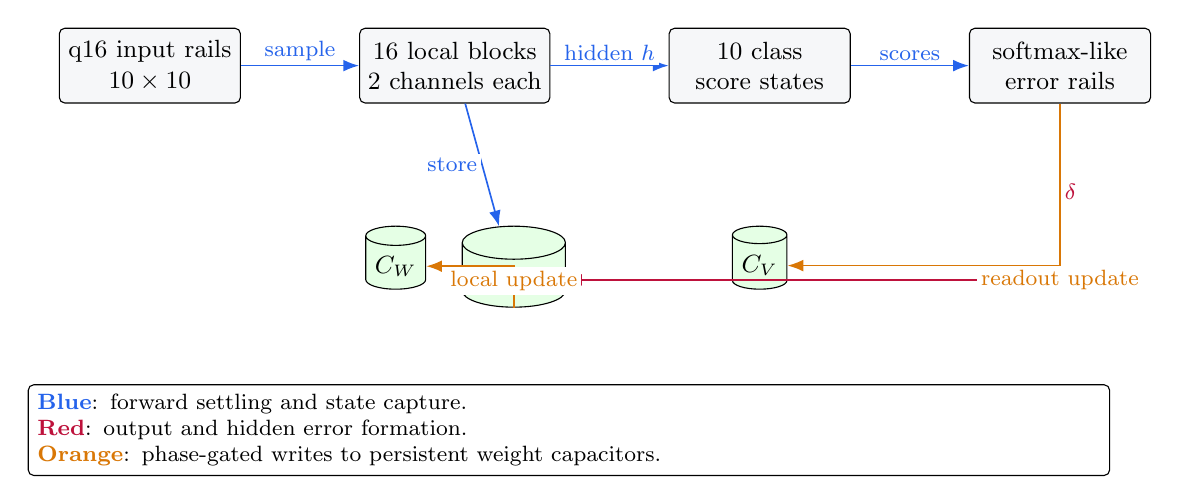
\begin{tikzpicture}[
      font=\small,
      block/.style={draw, rounded corners=2pt, minimum height=0.95cm,
        minimum width=2.3cm, align=center, fill=lightgray, inner sep=3pt},
      statecap/.style={draw, cylinder, shape border rotate=90, aspect=0.32,
        minimum height=0.8cm, minimum width=0.65cm, align=center, fill=green!10},
      arr/.style={-{Latex[length=2mm]}, semithick},
      fwd/.style={arr, forwardblue},
      bwd/.style={arr, backred},
      wr/.style={arr, writeorange},
      lbl/.style={font=\footnotesize, fill=white, inner sep=1.5pt}
    ]
    \node[block] (x) {q16 input rails\\\(10\times10\)};
    \node[block, right=1.5cm of x] (local) {16 local blocks\\2 channels each};
    \node[block, right=1.5cm of local] (scores) {10 class\\score states};
    \node[block, right=1.5cm of scores] (err) {softmax-like\\error rails};

    \node[statecap, below=1.55cm of local, xshift=-0.75cm] (w) {\(C_W\)};
    \node[statecap, below=1.55cm of local, xshift=0.75cm] (h) {\(C_h,C_{\delta h}\)};
    \node[statecap, below=1.55cm of scores] (v) {\(C_V\)};

    \draw[fwd] (x) -- node[lbl, above] {sample} (local);
    \draw[fwd] (local) -- node[lbl, above] {hidden \(h\)} (scores);
    \draw[fwd] (scores) -- node[lbl, above] {scores} (err);

    \draw[fwd] (local) -- node[lbl, left] {store} (h);
    \draw[backred, -{Latex[length=2mm]}, semithick] (err.south) |- node[lbl, right, pos=0.25] {\(\delta\)} (h.east);
    \draw[writeorange, -{Latex[length=2mm]}, semithick] (h.south) |- node[lbl, below] {local update} (w.east);
    \draw[writeorange, -{Latex[length=2mm]}, semithick] (err.south) |- node[lbl, below] {readout update} (v.east);

    \node[draw, rounded corners=2pt, fill=white, align=left,
      text width=13.5cm, below=1.2cm of w, xshift=2.2cm, font=\footnotesize]
      {\textcolor{forwardblue}{\textbf{Blue}}: forward settling and state
       capture.\\
       \textcolor{backred}{\textbf{Red}}: output and hidden error formation.\\
       \textcolor{writeorange}{\textbf{Orange}}: phase-gated writes to
       persistent weight capacitors.};
  \end{tikzpicture}
  \caption{Working local-feature/readout architecture.  The hidden block
  contains 32 local feature cells.  Persistent capacitor states hold local
  weights and biases, hidden activations and hidden deltas during a cycle, and
  class readout weights.  The high-accuracy behavioral run freezes output bias
  state, so there is no output-bias write path in that run.}
  \label{fig:working-architecture}
\end{figure}

\section{State And Update Equations}

The SPICE deck represents trainable state as capacitor voltages:
\[
  W_{bcp},\quad b_{bc},\quad V_{kbc},
\]
where \(b\) indexes a block position, \(c\) a local channel, \(p\) a pixel
inside the \(4\times4\) block, and \(k\) a class.  The final network has
\[
  16\cdot2\cdot16 = 512
\]
local weight states, 32 local bias states, and
\[
  10\cdot16\cdot2 = 320
\]
readout weight states.  Output biases are frozen in the high-accuracy
behavioral run, leaving 864 printed trainable state vectors.

For one sample, each local feature computes a block-local preactivation
\[
  z_{bc} = b_{bc} + \sum_p S_W(W_{bcp})\,x_{bp},
\]
then a hidden activation
\[
  h_{bc} = \tanh(z_{bc}).
\]
The best-performing branch uses a tanh-clipped transfer for local hidden
synapses,
\[
  S_W(w) = s \tanh(w/s),
\]
and a linear transfer for the class readout.  The class scores are
\[
  s_k = \sum_{b,c} V_{kbc}\,h_{bc} + o_k,
\]
with frozen \(o_k\) in the high-accuracy behavioral run.  The output error is
softmax-like:
\[
  d_k = t_k - \operatorname{softmax}(s/T)_k,
\]
with temperature \(T=2.0\).  Hidden deltas are local:
\[
  \delta h_{bc}
  =
  \left(\sum_k d_k\,V_{kbc}\right)
  (1-\tanh^2(z_{bc})).
\]

The phase-gated current sources implement direct online updates to the
capacitor voltages:
\[
  \Delta W_{bcp} = \eta\,\delta h_{bc}\,x_{bp},\qquad
  \Delta b_{bc} = \eta\,\delta h_{bc},
\]
\[
  \Delta V_{kbc} = \eta\,\alpha_V\,d_k\,h_{bc},
\]
with \(\alpha_V=0.5\) for the high-accuracy behavioral run.  These equations are rendered as
SPICE behavioral current terms into the state capacitors, gated by phase
clocks.  They are not computed by Python during the transient.  The behavioral
terms are the current stand-in for the transistor writer blocks; the important
architectural property of this result is continuous persistent state and local
phase-gated writes, not Python-side gradient application.

\section{Neuron Circuit Used In The Final Run}

The hidden neuron used in the \(90.15\%\) behavioral/local-PCA run is the stored tanh
local-feature cell shown in Fig.~\ref{fig:stored-tanh-neuron}.  It is precise
to the generated SPICE topology: the preactivation is an inline weighted sum,
the activation is stored on a capacitor during the activation phase, the hidden
delta is stored on a second capacitor during the backward phase, and the update
current sources read those stored node voltages during the write phase.

\begin{figure}[H]
  \centering
  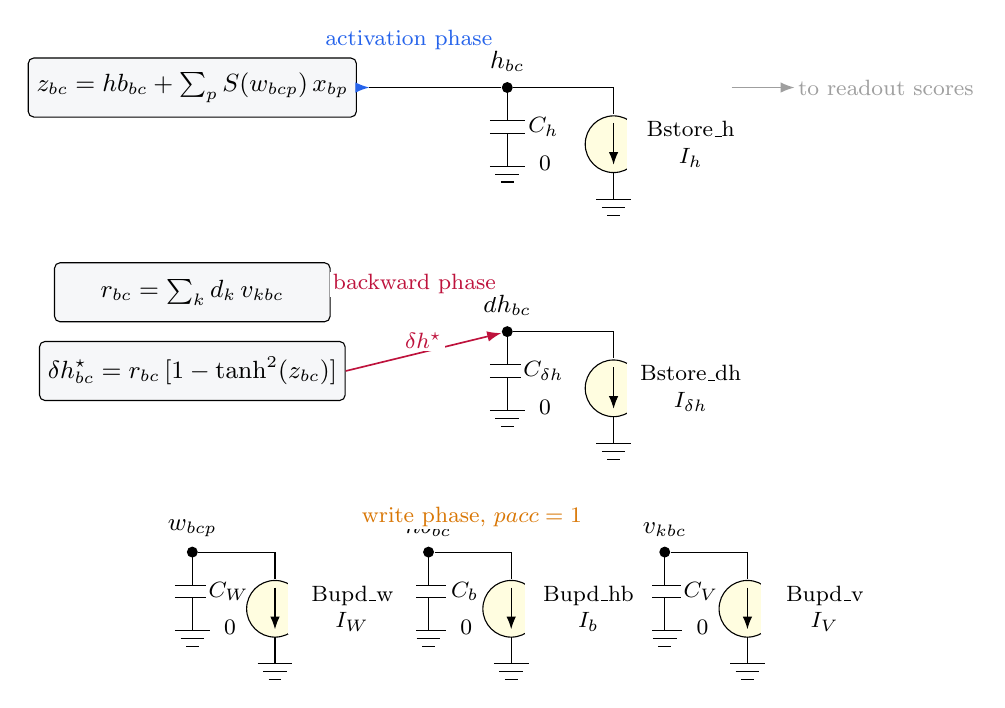
\begin{tikzpicture}[
      font=\small,
      expr/.style={draw, rounded corners=2pt, align=center, fill=lightgray,
        minimum width=3.5cm, minimum height=0.75cm, inner sep=3pt},
      rail/.style={font=\footnotesize, fill=white, inner sep=1pt},
      dot/.style={circle, fill=black, inner sep=1.4pt},
      bsrc/.style={circle, draw, minimum size=0.72cm, inner sep=0pt,
        fill=yellow!12},
      arr/.style={-{Latex[length=1.8mm]}, semithick},
      sig/.style={arr, gray!75},
      fwd/.style={arr, forwardblue},
      bwd/.style={arr, backred},
      wr/.style={arr, writeorange}
    ]
    \newcommand{\capgnd}[4]{%
      \draw (#1,#2) -- ++(0,-0.42);
      \draw (#1-0.22,#2-0.42) -- (#1+0.22,#2-0.42);
      \draw (#1-0.22,#2-0.58) -- (#1+0.22,#2-0.58);
      \draw (#1,#2-0.58) -- ++(0,-0.42);
      \draw (#1-0.22,#2-1.00) -- (#1+0.22,#2-1.00);
      \draw (#1-0.15,#2-1.10) -- (#1+0.15,#2-1.10);
      \draw (#1-0.08,#2-1.20) -- (#1+0.08,#2-1.20);
      \node[rail] at (#1+0.46,#2-0.50) {#3};
      \node[rail] at (#1+0.48,#2-0.96) {#4};
    }
    \newcommand{\isrcgnd}[5]{%
      \draw (#1,#2) -- ++(0,-0.34);
      \node[bsrc] (#5) at (#1,#2-0.72) {};
      \draw[-{Latex[length=1.6mm]}] (#1,#2-0.45) -- (#1,#2-0.98);
      \draw (#1,#2-1.08) -- ++(0,-0.34);
      \draw (#1-0.22,#2-1.42) -- (#1+0.22,#2-1.42);
      \draw (#1-0.15,#2-1.52) -- (#1+0.15,#2-1.52);
      \draw (#1-0.08,#2-1.62) -- (#1+0.08,#2-1.62);
      \node[rail, align=center, text width=1.55cm] at (#1+0.98,#2-0.72)
        {#3\\#4};
    }

    \node[expr] (zexpr) at (0,0.25)
      {\(z_{bc}=hb_{bc}+\sum_p S(w_{bcp})\,x_{bp}\)};
    \node[dot, label=above:\(h_{bc}\)] (hnode) at (4.0,0.25) {};
    \draw[fwd] (zexpr.east) -- (2.25,0.25);
    \draw (2.25,0.25) -- (hnode);
    \capgnd{4.0}{0.25}{\(C_h\)}{\(0\)}
    \isrcgnd{5.35}{0.25}{\(\mathrm{Bstore\_h}\)}
      {\(I_h\)}{Ih}
    \draw (hnode) -- (5.35,0.25);
    \draw[sig] (6.85,0.25) -- ++(0.8,0)
      node[rail, right] {to readout scores};
    \node[rail, text=forwardblue] at (2.75,0.85) {activation phase};

    \node[expr] (rexpr) at (0,-2.35)
      {\(r_{bc}=\sum_k d_k\,v_{kbc}\)};
    \node[expr] (dexpr) at (0,-3.35)
      {\(\delta h^\star_{bc}=r_{bc}\,[1-\tanh^2(z_{bc})]\)};
    \node[dot, label=above:\(dh_{bc}\)] (dhnode) at (4.0,-2.85) {};
    \draw[bwd] (dexpr.east) -- node[rail, above] {\(\delta h^\star\)}
      (dhnode);
    \capgnd{4.0}{-2.85}{\(C_{\delta h}\)}{\(0\)}
    \isrcgnd{5.35}{-2.85}{\(\mathrm{Bstore\_dh}\)}
      {\(I_{\delta h}\)}{Idh}
    \draw (dhnode) -- (5.35,-2.85);
    \node[rail, text=backred] at (2.82,-2.25) {backward phase};

    \node[dot, label=above:\(w_{bcp}\)] (wnode) at (0,-5.65) {};
    \node[dot, label=above:\(hb_{bc}\)] (hbnode) at (3.0,-5.65) {};
    \node[dot, label=above:\(v_{kbc}\)] (vnode) at (6.0,-5.65) {};
    \capgnd{0}{-5.65}{\(C_W\)}{\(0\)}
    \capgnd{3.0}{-5.65}{\(C_b\)}{\(0\)}
    \capgnd{6.0}{-5.65}{\(C_V\)}{\(0\)}
    \isrcgnd{1.05}{-5.65}{\(\mathrm{Bupd\_w}\)}
      {\(I_W\)}{Iw}
    \isrcgnd{4.05}{-5.65}{\(\mathrm{Bupd\_hb}\)}
      {\(I_b\)}{Ihb}
    \isrcgnd{7.05}{-5.65}{\(\mathrm{Bupd\_v}\)}
      {\(I_V\)}{Iv}
    \draw (wnode) -- (1.05,-5.65);
    \draw (hbnode) -- (4.05,-5.65);
    \draw (vnode) -- (7.05,-5.65);
    \node[rail, text=writeorange] at (3.55,-5.20) {write phase, \(pacc=1\)};
  \end{tikzpicture}
  \caption{Element-level schematic of one stored tanh hidden neuron and its
  attached write devices in the final SPICE deck.  The arrows inside the
  current-source symbols point from the named state node to ground, matching
  SPICE's \(\code{Bxxx node 0 I=...}\) branch-current convention.  Positive
  storage current therefore discharges the state capacitor; a negative write
  current injects charge and raises the stored weight voltage.}
  \label{fig:stored-tanh-neuron}
\end{figure}

The same circuit can be drawn in LTspice from the following deck stencil.  The
\(\sum_p\) in the comments is not a special SPICE primitive; for a concrete
cell it is expanded into one term per pixel in the block.  The signed weight
map \(S(\cdot)\) is the clipping/sign function used by the generated deck.
\[
\begin{array}{lll}
  h_{bc} &:& \text{stored activation node} \\
  dh_{bc} &:& \text{stored hidden-delta node} \\
  w_{bcp}, hb_{bc}, v_{kbc} &:&
    \text{local weight, local bias, and readout weight nodes} \\
  pact,pbwd,pacc &:&
    \text{nonoverlapping activation, backward, and write phase rails.}
\end{array}
\]

\begin{verbatim}
* One hidden local-feature neuron: block b, channel c.
* Expand zbc by writing one signed/clipped weight term per pixel p:
* zbc = V(hb_bc)
*     + S(V(w_bc0))*V(x_b0)
*     + S(V(w_bc1))*V(x_b1) + ...

Ch_bc        h_bc    0  {CSTATE} IC=0
Bstore_h_bc  h_bc    0  I = V(pact)*{CSTATE}/{TAU}*(V(h_bc)-tanh(zbc))

Cdh_bc       dh_bc   0  {CSTATE} IC=0
* rbc = sum_k V(d_k)*V(v_kbc)
* dh_target = rbc*(1-tanh(zbc)*tanh(zbc))
Bstore_dh_bc dh_bc   0  I = V(pbwd)*{CSTATE}/{TAU}*(V(dh_bc)-dh_target)

Cw_bcp       w_bcp   0  {CW} IC=<random_init>
Bupd_w_bcp   w_bcp   0  I = -V(pacc)*{CW}*eta*{LOCAL_UPDATE_SCALE}
+                         /({BS}*{TAREA})*V(dh_bc)*V(x_bp)

Chb_bc       hb_bc   0  {CW} IC=<random_init>
Bupd_hb_bc   hb_bc   0  I = -V(pacc)*{CW}*eta*{LOCAL_UPDATE_SCALE}
+                         /({BS}*{TAREA})*V(dh_bc)

Cv_kbc       v_kbc   0  {CW} IC=<random_init>
Bupd_v_kbc   v_kbc   0  I = -V(pacc)*{CW}*eta*{READOUT_UPDATE_SCALE}
+                         /({BS}*{TAREA})*V(d_k)*V(h_bc)
\end{verbatim}

In generated-deck form, the key hidden activation source is equivalent to
\[
  I_h =
  V(\mathrm{pact})\,\frac{C_{\mathrm{STATE}}}{\tau}
  \left[V(h_{bc})-\tanh(z_{bc})\right],
\]
which gives
\[
  \frac{dV(h_{bc})}{dt}
  =
  V(\mathrm{pact})\,\frac{\tanh(z_{bc})-V(h_{bc})}{\tau}.
\]
The hidden delta storage uses the same first-order form with target
\[
  \left(\sum_k d_kV_{kbc}\right)(1-\tanh^2(z_{bc})).
\]
This is the circuit actually used by the high-accuracy behavioral/local-PCA
run.  Earlier MOS ReLU and differential source-follower cells remain important
transistor-level building blocks, but they have not yet replaced this
behavioral neuron/write kernel in a high-accuracy run.

\section{Trainable Cell Catalog}

The repository now treats a hidden block/channel as a
\(\code{TrainableDynamicalCell}\): a circuit-emittable learning object with
public input/output/learning ports, declared internal state, a learning
protocol, and characterization expectations.  The first ten concrete cells are
behavioral local-feature candidates.  They all share the same state and phase
contract shown in Fig.~\ref{fig:cell-template}; they differ in the forward
nonlinearity \(\phi\), the hidden synapse transfer \(S_W\), the derivative
gate, and the hidden-error feedback path.

\begin{figure}[H]
  \centering
  \resizebox{\linewidth}{!}{%
  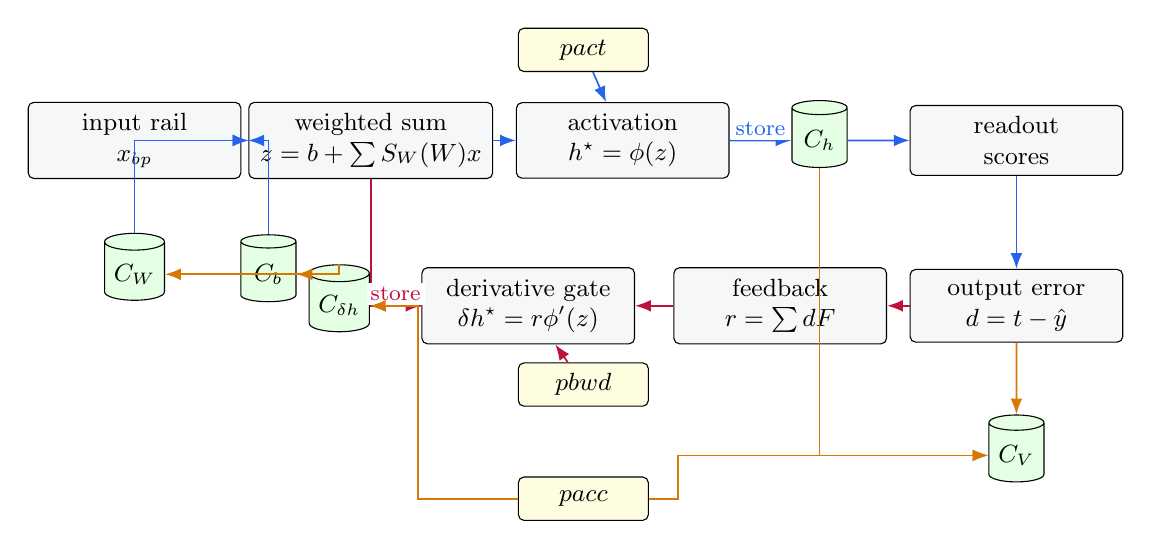
\begin{tikzpicture}[
      font=\small,
      box/.style={draw, rounded corners=2pt, align=center, fill=lightgray,
        minimum width=2.7cm, minimum height=0.85cm, inner sep=4pt},
      statecap/.style={draw, cylinder, shape border rotate=90, aspect=0.28,
        minimum width=0.7cm, minimum height=0.85cm, fill=green!10,
        align=center},
      phase/.style={draw, rounded corners=2pt, align=center, fill=yellow!12,
        minimum width=1.65cm, minimum height=0.55cm, inner sep=2pt},
      arr/.style={-{Latex[length=2mm]}, semithick},
      fwd/.style={arr, forwardblue},
      bwd/.style={arr, backred},
      wr/.style={arr, writeorange},
      lbl/.style={font=\footnotesize, fill=white, inner sep=1.5pt}
    ]
    \node[box] (x) at (0,0) {input rail\\\(x_{bp}\)};
    \node[statecap] (w) at (0,-1.7) {\(C_W\)};
    \node[statecap] (b) at (1.7,-1.7) {\(C_b\)};
    \node[box] (sum) at (3.0,0) {weighted sum\\\(z=b+\sum S_W(W)x\)};
    \node[box] (phi) at (6.2,0) {activation\\\(h^\star=\phi(z)\)};
    \node[statecap] (h) at (8.7,0) {\(C_h\)};
    \node[box] (score) at (11.2,0) {readout\\scores};

    \node[box] (err) at (11.2,-2.1) {output error\\\(d=t-\hat y\)};
    \node[box] (fb) at (8.2,-2.1) {feedback\\\(r=\sum dF\)};
    \node[box] (gate) at (5.0,-2.1) {derivative gate\\\(\delta h^\star=r\phi'(z)\)};
    \node[statecap] (dh) at (2.6,-2.1) {\(C_{\delta h}\)};
    \node[statecap] (v) at (11.2,-4.0) {\(C_V\)};

    \node[phase] (pact) at (5.7,1.15) {\(pact\)};
    \node[phase] (pbwd) at (5.7,-3.1) {\(pbwd\)};
    \node[phase] (pacc) at (5.7,-4.55) {\(pacc\)};

    \draw[fwd] (x) -- (sum);
    \draw[fwd] (w) |- (sum);
    \draw[fwd] (b) |- (sum);
    \draw[fwd] (sum) -- (phi);
    \draw[fwd] (phi) -- node[lbl, above] {store} (h);
    \draw[fwd] (h) -- (score);
    \draw[fwd] (score) -- (err);

    \draw[bwd] (err) -- (fb);
    \draw[bwd] (fb) -- (gate);
    \draw[bwd] (sum) |- (gate);
    \draw[bwd] (gate) -- node[lbl, above] {store} (dh);

    \draw[wr] (dh) |- (w);
    \draw[wr] (dh) |- (b);
    \draw[wr] (err) -- (v);
    \draw[wr] (h) |- (v);

    \draw[fwd] (pact) -- (phi);
    \draw[bwd] (pbwd) -- (gate);
    \draw[wr] (pacc) -- (6.9,-4.55) |- (v);
    \draw[wr] (pacc) -- (3.6,-4.55) |- (dh);
  \end{tikzpicture}}
  \caption{Common local-feature cell template used by the ten behavioral
  candidates.  Forward state \(h\), backward state \(\delta h\), local weights
  and biases, and readout weights are capacitor states.  Candidate cells
  replace the activation, synapse transfer, derivative gate, and feedback
  block while preserving the same public-port and phase contract.}
  \label{fig:cell-template}
\end{figure}

\begin{figure}[H]
  \centering
  \resizebox{\linewidth}{!}{%
  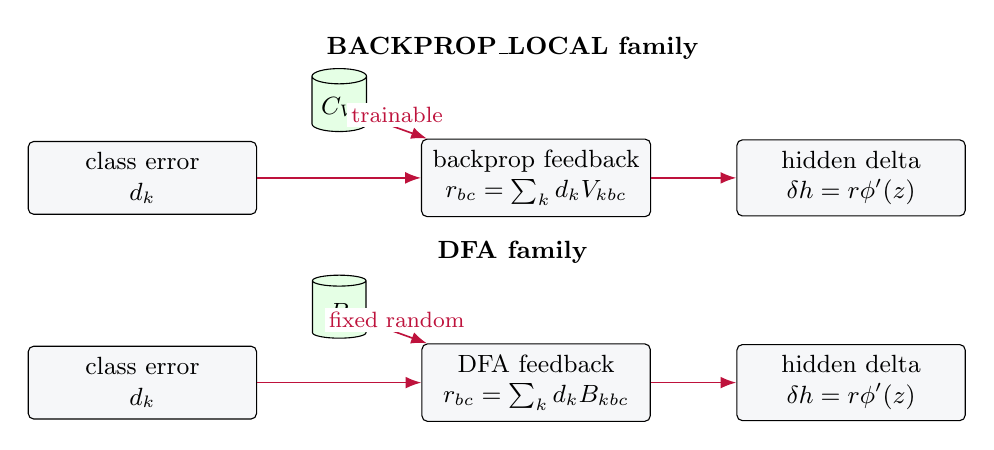
\begin{tikzpicture}[
      font=\small,
      box/.style={draw, rounded corners=2pt, align=center, fill=lightgray,
        minimum width=2.9cm, minimum height=0.82cm, inner sep=4pt},
      statecap/.style={draw, cylinder, shape border rotate=90, aspect=0.28,
        minimum width=0.68cm, minimum height=0.8cm, fill=green!10,
        align=center},
      arr/.style={-{Latex[length=2mm]}, semithick},
      fwd/.style={arr, forwardblue},
      bwd/.style={arr, backred},
      lbl/.style={font=\footnotesize, fill=white, inner sep=1.5pt}
    ]
    \node[box] (err1) at (0,0) {class error\\\(d_k\)};
    \node[statecap] (v1) at (2.5,0.9) {\(C_V\)};
    \node[box] (fb1) at (5.0,0) {backprop feedback\\\(r_{bc}=\sum_k d_kV_{kbc}\)};
    \node[box] (dh1) at (9.0,0) {hidden delta\\\(\delta h=r\phi'(z)\)};
    \draw[bwd] (err1) -- (fb1);
    \draw[bwd] (v1) -- node[lbl, above] {trainable} (fb1);
    \draw[bwd] (fb1) -- (dh1);
    \node[font=\bfseries\small] at (4.7,1.65) {BACKPROP\_LOCAL family};

    \node[box] (err2) at (0,-2.6) {class error\\\(d_k\)};
    \node[statecap] (b2) at (2.5,-1.7) {\(B\)};
    \node[box] (fb2) at (5.0,-2.6) {DFA feedback\\\(r_{bc}=\sum_k d_kB_{kbc}\)};
    \node[box] (dh2) at (9.0,-2.6) {hidden delta\\\(\delta h=r\phi'(z)\)};
    \draw[bwd] (err2) -- (fb2);
    \draw[bwd] (b2) -- node[lbl, above] {fixed random} (fb2);
    \draw[bwd] (fb2) -- (dh2);
    \node[font=\bfseries\small] at (4.7,-0.95) {DFA family};
  \end{tikzpicture}}
  \caption{Backward-path variants.  Most catalog cells use the trainable
  readout weights as the feedback path, possibly clipped or sign-compressed.
  The DFA cell keeps the same forward and write machinery but replaces
  transposed readout feedback with a fixed random projection.}
  \label{fig:cell-feedback}
\end{figure}

Figure~\ref{fig:cell-transfer-families} shows the circuit meaning of the main
candidate families.  These are still behavioral cells: each transfer is emitted
as a mathematical SPICE expression today, then promoted to a transistor
candidate only if the replacement passes update-alignment and disturb tests.

\begin{figure}[H]
  \centering
  \resizebox{\linewidth}{!}{%
  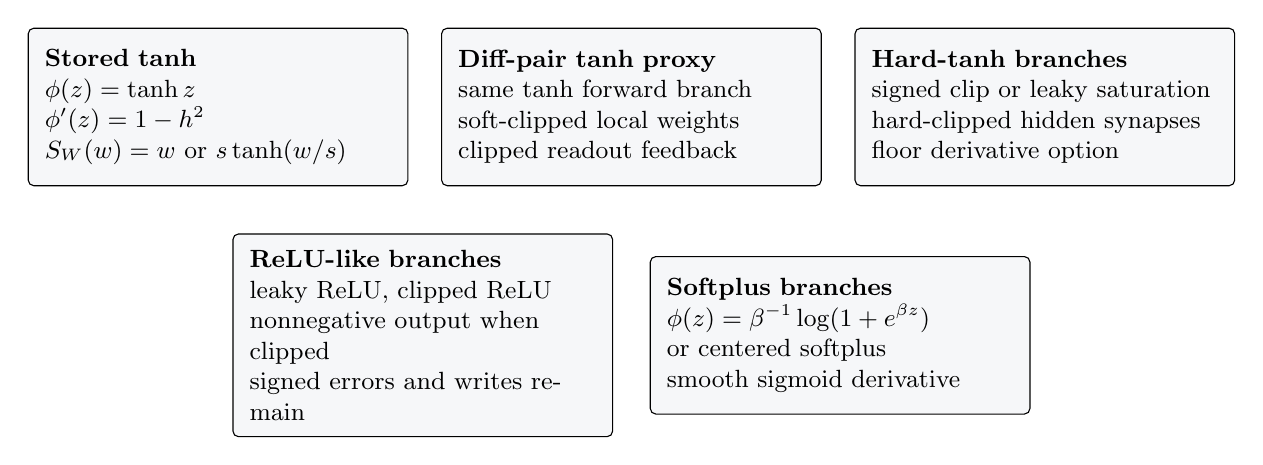
\begin{tikzpicture}[
      font=\small,
      fam/.style={draw, rounded corners=2pt, align=left, fill=lightgray,
        text width=4.4cm, minimum height=2.0cm, inner sep=6pt}
    ]
    \node[fam] (tanh) at (0,0) {
      \textbf{Stored tanh}\\
      \(\phi(z)=\tanh z\)\\
      \(\phi'(z)=1-h^2\)\\
      \(S_W(w)=w\) or \(s\tanh(w/s)\)
    };
    \node[fam] (diff) at (5.25,0) {
      \textbf{Diff-pair tanh proxy}\\
      same \(\tanh\) forward branch\\
      soft-clipped local weights\\
      clipped readout feedback
    };
    \node[fam] (hard) at (10.5,0) {
      \textbf{Hard-tanh branches}\\
      signed clip or leaky saturation\\
      hard-clipped hidden synapses\\
      floor derivative option
    };
    \node[fam] (relu) at (2.6,-2.9) {
      \textbf{ReLU-like branches}\\
      leaky ReLU, clipped ReLU\\
      nonnegative output when clipped\\
      signed errors and writes remain
    };
    \node[fam] (soft) at (7.9,-2.9) {
      \textbf{Softplus branches}\\
      \(\phi(z)=\beta^{-1}\log(1+e^{\beta z})\)\\
      or centered softplus\\
      smooth sigmoid derivative
    };
  \end{tikzpicture}}
  \caption{Transfer-function families represented in the ten-cell catalog.
  The strongest first smoke was the differential-pair-inspired tanh/soft-clip
  branch, which is attractive because a MOS differential pair naturally gives a
  tanh-like transfer and soft saturation.}
  \label{fig:cell-transfer-families}
\end{figure}

All ten catalog cells use the same online local-learning skeleton:
\[
  z_{bc}=b_{bc}+\sum_p S_W(W_{bcp})\,x_{bp},
  \qquad
  h_{bc}=\phi(z_{bc}),
\]
\[
  s_k=\sum_{b,c}S_V(V_{kbc})\,h_{bc}+o_k,
  \qquad
  d_k=t_k-\operatorname{softmax}(s/T)_k,
\]
\[
  r_{bc}=\sum_k d_k F_{kbc},
  \qquad
  \delta h_{bc}=r_{bc}\,g(z_{bc},h_{bc}),
\]
\[
  \Delta W_{bcp}=\eta\,\delta h_{bc}x_{bp},
  \qquad
  \Delta b_{bc}=\eta\,\delta h_{bc},
  \qquad
  \Delta V_{kbc}=\eta\,\alpha_V d_k h_{bc}.
\]
The cell-specific choices are the activation \(\phi\), derivative gate \(g\),
hidden synapse transfer \(S_W\), readout transfer \(S_V\), and feedback matrix
\(F\).  The common transfer primitives are:
\[
  S_{\mathrm{linear}}(w)=w,\qquad
  S_{\mathrm{tanhclip}}(w;s)=s\tanh(w/s),\qquad
  S_{\mathrm{hardclip}}(w;s)=\operatorname{clip}(w,-s,s),
\]
\[
  F_{\mathrm{readout}}=S_V(V),\qquad
  F_{\mathrm{clip}}=c\tanh(S_V(V)/c),\qquad
  F_{\mathrm{DFA}}=B_{\mathrm{fixed}}.
\]

\begin{table}[H]
  \centering
  \caption{Governing equations for the ten catalog cells.  These are the
  equations exercised by the unit characterization and by the NumPy MNIST
  benchmark.}
  \label{tab:cell-equations}
  \scriptsize
  \begin{tabular}{>{\raggedright\arraybackslash}p{0.23\linewidth}
                  >{\raggedright\arraybackslash}p{0.27\linewidth}
                  >{\raggedright\arraybackslash}p{0.27\linewidth}
                  >{\raggedright\arraybackslash}p{0.14\linewidth}}
    \toprule
    Cell & Forward activation \(\phi(z)\) and gate \(g\) & Synapse/feedback equations & Unit validation \\
    \midrule
    \code{stored\_tanh\_tanhclip} &
    \(\phi=\tanh z,\; g=1-h^2\) &
    \(S_W=S_{\mathrm{tanhclip}}(w;1.0),\; S_V(w)=w,\; F=V,\; \alpha_V=0.5\) &
    monotone; \(g\ge0\); update sign/cosine aligned \\
    \addlinespace
    \code{stored\_tanh\_linear} &
    \(\phi=\tanh z,\; g=1-h^2\) &
    \(S_W(w)=w,\; S_V(w)=w,\; F=V\) &
    monotone; \(g\ge0\); update sign/cosine aligned \\
    \addlinespace
    \code{diffpair\_tanh\_softclip} &
    \(\phi=\tanh z,\; g=1-h^2\) &
    \(S_W=S_{\mathrm{tanhclip}}(w;0.75),\; S_V(w)=w,\; F=0.25\tanh(V/0.25)\) &
    monotone; \(g\ge0\); update sign/cosine aligned \\
    \addlinespace
    \code{signed\_hardtanh} &
    \(\phi=\operatorname{clip}(z,-1,1),\;
      g=\mathbf{1}_{|z|\le1}\) &
    \(S_W=S_{\mathrm{hardclip}}(w;1.0),\; S_V(w)=w,\; F=V\) &
    monotone; \(g\ge0\); update sign/cosine aligned \\
    \addlinespace
    \code{leaky\_hardtanh} &
    \(\phi=z\) for \(|z|\le1\), else
    \(\operatorname{sign}(z)(1+0.05(|z|-1))\);
    \(g=0.02+0.98\,[\mathbf{1}_{|z|\le1}\vee0.05]\) &
    \(S_W=S_{\mathrm{hardclip}}(w;1.0),\; S_V(w)=w,\; F=V\) &
    monotone; \(g\ge0\); update sign/cosine aligned \\
    \addlinespace
    \code{leaky\_relu} &
    \(\phi=\max(z,0)+0.05\min(z,0),\;
      g=1\) for \(z\ge0\), \(0.05\) otherwise &
    \(S_W=S_{\mathrm{tanhclip}}(w;1.0),\; S_V(w)=w,\; F=V\) &
    monotone; \(g\ge0\); update sign/cosine aligned \\
    \addlinespace
    \code{clipped\_relu} &
    \(\phi=\operatorname{clip}(z,0,1),\;
      g=0.02+0.98\mathbf{1}_{0\le z\le1}\) &
    \(S_W=S_{\mathrm{tanhclip}}(w;1.0),\; S_V(w)=w,\; F=V\) &
    monotone; \(g\ge0\); update sign/cosine aligned \\
    \addlinespace
    \code{softplus} &
    \(\phi=\beta^{-1}\log(1+e^{\beta z}),\;
      g=(1+e^{-\beta z})^{-1},\; \beta=4\) &
    \(S_W=S_{\mathrm{tanhclip}}(w;1.0),\; S_V(w)=w,\; F=V\) &
    monotone; \(g\ge0\); update sign/cosine aligned \\
    \addlinespace
    \code{centered\_softplus} &
    \(\phi=\beta^{-1}[\log(1+e^{\beta z})-\log2],\;
      g=(1+e^{-\beta z})^{-1},\; \beta=4\) &
    \(S_W=S_{\mathrm{tanhclip}}(w;1.0),\; S_V(w)=w,\; F=V\) &
    monotone; \(g\ge0\); update sign/cosine aligned \\
    \addlinespace
    \code{dfa\_tanh\_fixed\_feedback} &
    \(\phi=\tanh z,\; g=1-h^2\) &
    \(S_W=S_{\mathrm{tanhclip}}(w;1.0),\; S_V(w)=w,\; F=B_{\mathrm{fixed}}\) &
    monotone; \(g\ge0\); update sign/cosine aligned \\
    \bottomrule
  \end{tabular}
\end{table}

The automated tests validate the equations at the contract and single-cell
levels.  The contract-validity test checks that all ten cells declare valid
ports, signedness, state roles, and protocol requirements.  The
learning-alignment test runs the characterization equations over a
deterministic operating grid:
\(\phi(z)\) must be monotone on \(z\in[-2.5,2.5]\), the derivative gate must be
nonnegative, the hidden synapse transfer must remain finite on
\([-4,4]\), and the synthetic local update must have positive cosine and
perfect sign alignment with the reference rule
\[
  \operatorname{sign}(\Delta W)=\operatorname{sign}(\delta h\,x).
\]
The MNIST benchmark then experimentally exercises the same equations in a
small online classifier.  It is a real-data behavioral smoke, not a SPICE or
transistor validation.

\begin{table}[H]
  \centering
  \caption{Ten behavioral local-feature cells and their real-MNIST smoke
  result.  The benchmark used \(10\times10\), block 4, stride 2, 2 channels,
  q16 inputs, 512 online updates, 1000 evaluation images, seeded random order,
  and no local-PCA.}
  \label{tab:cell-catalog}
  \scriptsize
  \begin{tabular}{llllr}
    \toprule
    Cell & Activation & Hidden synapse & Feedback path & Final acc. \\
    \midrule
    \code{diffpair\_tanh\_softclip} & tanh & tanh-clipped, \(s=0.75\) & clipped readout & \(56.6\%\) \\
    \code{dfa\_tanh\_fixed\_feedback} & tanh & tanh-clipped & fixed random \(B\) & \(54.2\%\) \\
    \code{stored\_tanh\_tanhclip} & tanh & tanh-clipped & readout & \(50.4\%\) \\
    \code{stored\_tanh\_linear} & tanh & linear & readout & \(46.1\%\) \\
    \code{leaky\_relu} & leaky ReLU & tanh-clipped & readout & \(42.7\%\) \\
    \code{softplus} & softplus & tanh-clipped & readout & \(41.8\%\) \\
    \code{centered\_softplus} & centered softplus & tanh-clipped & readout & \(38.3\%\) \\
    \code{clipped\_relu} & clipped ReLU & tanh-clipped & readout & \(37.8\%\) \\
    \code{leaky\_hardtanh} & leaky hard-tanh & hard-clipped & readout & \(35.8\%\) \\
    \code{signed\_hardtanh} & signed hard clip & hard-clipped & readout & \(24.6\%\) \\
    \bottomrule
  \end{tabular}
\end{table}

This catalog changes the promotion strategy.  Instead of replacing the working
stored tanh neuron with an arbitrary transistor ReLU, each candidate must keep
the same cell contract and prove four local properties before a full SPICE
MNIST run: monotone forward transfer, nonnegative derivative gate over the
declared operating range, signed update alignment, and acceptable state hold
and read disturb.  The current best promotion target is
\(\code{diffpair\_tanh\_softclip}\), because it both ranked first in the real
MNIST behavioral smoke and maps naturally onto a differential-pair
implementation.

\section{Phase Schedule}

The runner uses a repeated sample cycle with separate guide rails for forward
settling, activation storage, score storage, error/backward formation, and
direct accumulation/write.  In the high-accuracy behavioral run the update is
direct:
there are no gradient-accumulator capacitors and no apply-once batch phase.
This is why the run uses \(\mathrm{batch\_size}=1\) and 6000 distinct online
updates.

Pulse-gated clocks were used instead of listing every clock edge as long PWL
tables.  Non-constant learning rate was also moved into an analytic in-deck
control expression:
\[
  \eta(n): 0.3 \rightarrow 0.06
\]
by linear decay over the 6000 updates.  These are source-complexity reductions,
not training shortcuts: the deck still sees time-varying control rails, while
the neural state remains inside SPICE.

\section{Signed Quantities}

A ReLU activation can be single-ended and nonnegative after rectification, but
the working system still needs signed transport in several places.  Synapse
contributions, preactivations, errors, hidden deltas, and weight updates are
signed.  The clean physical representation is therefore differential or
equivalent positive/negative storage for those quantities:
\[
  u = u^+ - u^-,
  \qquad
  \Delta w = \Delta w^+ - \Delta w^-.
\]
Positive-weight branches contribute to the positive summing rail and
negative-weight branches contribute to the negative summing rail.  Backward
error rails and update rails follow the same rule.

The final high-accuracy local-feature run uses tanh hidden activations rather
than a literal ReLU.  The design lesson from the neuron/synapse screens is
still the same: rectification can simplify activation outputs, but it does not
remove signed transport from the synapse, score, error, hidden-delta, or write
paths.  In the q16 target-topology screens, tanh hidden activations with
tanh-clipped local synapses were more robust than leaky ReLU, softplus, and
differential clipped-ReLU alternatives at the longer online horizons.

\section{Input And Source-Cost Choices}

The current deck includes source-cost optimizations that preserve the execution
contract, but not all of them are acceptable for the final goal.

\paragraph{q16 input rails.}
The \(10\times10\) input pixels are quantized to 16 levels before waveform
generation.  Python is still only driving input rails; it is not computing
network state.  Quantization reduces the number of source transitions while
preserving enough accuracy headroom for the high-accuracy branch.

\paragraph{Rejected local-PCA sample order.}
The \(90.15\%\) run used a local-PCA ordering inside 512-sample windows to
reduce input PWL switching.  Although this does not read or write neural state,
it is still an unrealistic training assumption: the data stream is chosen using
a structure-aware preprocessing pass whose purpose is simulator convenience.
It should therefore not count toward the final goal.  Future headline runs
should use the stable dataset order, a seeded random order, or another
training-realistic order that is chosen independently of source-waveform
compression.

\section{Current Evidence}

No final-goal result is claimed yet.  Table~\ref{tab:headline} records the
strongest high-accuracy run because it is useful architectural evidence, but it
is disqualified from the final objective for two reasons: the neuron/write cells
are behavioral current equations, and the training order uses local-PCA source
compression.  The compact artifacts are:
\begin{center}
\small
\path{results/tables/spice_mnist_local_feature_phase_codex_q16_6k_localpca512_strict_u6000_eval10k_summary.json}
\end{center}
and its corresponding equivalence/metrics CSV.

\begin{table}[H]
  \centering
  \caption{High-accuracy behavioral/local-PCA run.  This is evidence, not a
  final-goal result.}
  \label{tab:headline}
  \begin{tabular}{ll}
    \toprule
    Field & Value \\
    \midrule
    Simulator & Xyce 7.10 \\
    Architecture & phase-resolved transient local-feature readout \\
    Topology & \(10\times10\), block 4, stride 2, 2 channels \\
    Classes & 10 \\
    Train samples / updates & 6000 / 6000 \\
    Batch size & 1 \\
    Eval samples & 10,000 MNIST test images \\
    Initial eval accuracy & \(10.89\%\) \\
    Final eval accuracy & \(\mathbf{90.15\%}\) \\
    Improvement & \(+79.26\) percentage points \\
    Reference mode & none \\
    Python weight updates between samples & false \\
    Python checkpointing between samples & false \\
    Random initialization & true \\
    Execution contract met & true \\
    Final-goal status & disqualified: behavioral writers and local-PCA order \\
    \bottomrule
  \end{tabular}
\end{table}

\begin{table}[H]
  \centering
  \caption{Key knobs and simulation cost for the disqualified high-accuracy
  run.}
  \label{tab:cost}
  \begin{tabular}{ll}
    \toprule
    Field & Value \\
    \midrule
    Input mode & PWL, 16 quantization levels \\
    Train order & local-PCA, window 512, not final-goal acceptable \\
    Hidden activation / local synapse & tanh / tanh-clipped \\
    Readout synapse & linear \\
    Learning rate & 0.3, linear decay to \(0.2\times\) \\
    LR control & analytic in-deck expression \\
    Readout update scale & 0.5 \\
    Output bias update scale & 0.0, frozen \\
    Softmax temperature & 2.0 \\
    Phase clock mode & pulse-gated \\
    Hidden activation/delta state & stored / stored \\
    Score/output delta state & stored / node \\
    Auxiliary algebraic source count & 0 \\
    Printed state vectors & 864 \\
    Estimated transient points & 16,803 \\
    Total source PWL points & 475,007 \\
    Pixel source PWL points & 465,518 \\
    Target source PWL points & 9,489 \\
    Phase wall time & 4,884.4 s \\
    \bottomrule
  \end{tabular}
\end{table}

\section{Design Evidence}

The current architecture was selected by bounded screens and strict promotions,
but the useful conclusions are short:
\begin{enumerate}
  \item A tiny \(4\times4\), block-2, stride-2, 1-channel transient verified
    continuous-state correctness: a one-transient online SPICE run matched the
    trusted batch-op update direction without Python checkpointing.
  \item The target \(10\times10\), block-4, stride-2, 2-channel topology was
    the best balance of feature capacity, state count, and strict transient
    cost.
  \item Tanh hidden units with tanh-clipped local synapses were the most robust
    long-horizon branch among the tested neuron/synapse choices.  Differential
    clipped-ReLU was competitive early but trailed at longer horizons; softplus
    and leaky ReLU were weaker in this setup.
  \item q16 input quantization reduced waveform pressure while preserving
    learning.  Local-PCA ordering reduced waveform pressure further, but it is
    now treated as a disallowed simulator convenience rather than a valid
    training assumption.
  \item Pulse-gated clocks and analytic LR control removed avoidable PWL
    sources.  Pixel input transitions remain the dominant source-cost term.
  \item The 1024-update and 2048-update strict promotions showed meaningful
    full-test learning under the execution contract.  The 6000-update run
    showed that the architecture has enough learning headroom to reach
    \(90.15\%\), but it does not close the final objective because of the
    behavioral writer/neuron cells and local-PCA order.
\end{enumerate}

The most important enablers were not any single magic neuron.  They were the
combination of (1) enough local feature capacity in the \(10\times10\),
block-4, stride-2, 2-channel topology; (2) a stable signed update rule with
stored hidden activations and hidden deltas; (3) tanh/tanh-clipped nonlinearities
that avoided the dead/one-sided behavior seen in several ReLU-like screens;
(4) frozen output bias, readout scale \(0.5\), and softmax temperature \(2.0\),
which kept the output error and readout writes in a useful range; and (5) source
compression that made the long strict transient runnable.  The local-PCA part
of that compression is not acceptable for the final result.

\section{What The Result Does And Does Not Claim}

The current evidence establishes that a high-performing SPICE training path can
be moved from Python-orchestrated checkpoint/update chunks into a continuous,
stateful SPICE simulation for the local-feature architecture.  The
high-accuracy run starts from random weights, performs online updates inside
one transient, and crosses \(90\%\) on full MNIST test accuracy.

It does not establish the final goal.  First, the update cells in this deck are
behavioral current equations standing in for the transistor writer blocks that
earlier device-level experiments explored.  Second, the \(90.15\%\) run used
local-PCA sample ordering, which should be removed from the headline path
because it is not a realistic training assumption.  A future device-level
version should preserve the same execution contract while replacing the
behavioral kernels with characterized MOS differential synapses, error rails,
and signed write branches, and while training under a realistic sample order.

\section{Training Faster And Scaling Further}

The main open problem is still the full objective: device-level training,
realistic sample order, one uninterrupted transient, \(\mathrm{batch\_size}=1\),
and \(>90\%\) full-test MNIST accuracy.  Cost is the immediate practical
blocker.  The disqualified 6000-update run spent most of its source complexity
on pixel waveforms: 465,518 of 475,007 PWL points came from pixel sources.
That makes the first speed target input delivery, not the number of printed
state vectors.

\paragraph{Near-term simulation speedups.}
The most plausible speedups are:
\begin{enumerate}
  \item replace per-pixel PWL rails with a simulator-friendly encoded input
    source or sample-and-hold front end;
  \item replace the local-PCA source-compression trick with realistic input
    compression that is independent of the sample ordering;
  \item avoid printing or measuring any state not needed for final diagnostics;
  \item use strict small-horizon equivalence runs to validate knobs before
    spending multi-thousand-update Xyce runs;
  \item keep analytic controls and pulse-gated clocks, since explicit PWL
    control rails add cost without adding learning value.
\end{enumerate}

\paragraph{Architecture scale-up.}
The state count for the private local-feature family scales as
\[
  N_{\mathrm{state}}
  \approx
  B C(P+1) + KBC,
\]
where \(B\) is the number of block positions, \(C\) channels, \(P\) pixels per
block, and \(K\) classes.  Increasing image size, reducing stride, or adding
channels therefore grows both local feature state and readout state.  Scaling
should be done by a Pareto ladder: increase one axis at a time, require a cheap
reference endpoint above target, then promote only bounded strict SPICE runs.

\paragraph{Circuit scale-up.}
The behavioral neuron/write kernels should be replaced by transistor-level
blocks only after the replacement passes three local tests:
\begin{enumerate}
  \item forward transfer matches the stored tanh or chosen replacement over
    the operating voltage range;
  \item backward delta transport has positive alignment with the reference
    hidden delta;
  \item signed write currents move \(C_W\) and \(C_b\) in the same direction as
    \(\delta h\,x\) without excessive read disturb or rail pinning.
\end{enumerate}

Only after those local tests pass should the transistor cell replace the
behavioral current kernel in a full MNIST strict transient.  Otherwise the
system will be debugging device nonidealities and architecture scaling at the
same time.

\end{document}
